\chapter{Asking Millionaires How They Got Rich (Austin)}

This chapter reads less like a formal blackboard lecture than like a field notebook written under pressure: we are taken from one entrepreneur to the next, given a number, and then asked for the mechanism that sits behind it. The numbers are not all of the same kind. Some refer to revenue, some to personal earnings, some to capital raised, some to valuation, some to exit price, and some to assets under management. If we keep those scales distinct, the episode becomes much clearer. What at first looks like a montage of wealth turns out to be a sequence of arguments about pricing, feedback, compounding, alignment, funding, and teams.

\begin{remark}
No validated board or slide frames survive from this lecture. The displayed equations below are therefore transcript-backed bookkeeping relations or cautious reconstructions of arithmetic stated verbally in the interviews.
\end{remark}

\section{Cold Open: A City Seen Through Numbers}

The lecture begins in fragments. One speaker says he made most of his net worth in e-commerce. Another says he ended up in high tech. A third says a business will revenue about $\$30$ million. Another says he made about $\$11.2$ million in a single year. Another mentions $\$87$ million raised, another a valuation of about $\$1$ billion, another a first company sold for about $\$150$ million. Only after this barrage does the host tell us where we are and what the point is: Austin is one of the fastest-growing cities in the country, rich in entrepreneurs, and the plan is to ask how wealth is actually built there.

\begin{definition}
For the rest of the chapter we distinguish the following objects:
\begin{itemize}
\item \(R\): company revenue,
\item \(E_{\text{year}}\): personal earnings in a year,
\item \(P_{\text{day,max}}\): a peak daily take,
\item \(C_{\text{raised}}\): outside capital raised,
\item \(V\): company valuation,
\item \(X\): exit or transaction value,
\item \(A_{\text{RE}}\): assets under management in real estate,
\item \(V_{\text{RE,proj}}\): projected developed value.
\end{itemize}
\end{definition}

The teaser itself can be read as a quick taxonomy of those scales:
\begin{align}
R &\approx \$30\,\text{million}, &
E_{\text{year}} &\approx \$11.2\,\text{million}, \\
C_{\text{raised}} &\approx \$87\,\text{million}, &
V &\approx \$1\,\text{billion}, \\
X_{\text{first exit}} &\approx \$150\,\text{million}. &&
\end{align}

The lecture is already making a quiet point. Wealth is not one number. Before we are allowed to ask how people got rich, we are forced to ask what kind of number we are even looking at.

\section{Josh: Short Bursts of Profit and the Problem of Price}

The first sustained case is Josh. The host arrives, admires the Lamborghini, and asks the simplest possible question: what industry are you in? Josh's answer gives us the base coordinates of the case. He is primarily an e-commerce entrepreneur, started in 2015, with real estate as a secondary domain. Then, as throughout the episode, the host immediately asks for magnitude:
\begin{align}
E_{\text{year}} &\approx \$11.2\,\text{million},\\
P_{\text{day,max}} &\approx \$1\,\text{million}.
\end{align}

The real interest lies in the second claim. Josh says, in effect, that very large sums may arrive in short windows. He contrasts the long slow grind of ordinary income with the sharp profits that come from launches, promotions, joint ventures, and concentrated marketing. If we want a compact proxy for what he calls a higher ``velocity to profit,'' we may write
\begin{equation}
v_P=\frac{\Delta P}{\Delta t},
\end{equation}
where \(\Delta P\) is the incremental profit captured over a campaign window \(\Delta t\). This formula is not spoken in the interview; it is a cautious way to formalize the contrast he is making between ordinary flow and concentrated payoff.

That contrast matters because it changes the rhythm of the question. We are no longer asking only how much was made. We are asking under what temporal structure it became possible.

\subsection{Question \& Answer}

\paragraph{Question.} How can a business charge more and still grow?

\paragraph{Answer.} Josh answers with the acronym WWAD: ``What Would Apple Do?'' He uses Apple to attack a common misconception, namely that there is some necessary opposition between charging a premium and growing fast. Apple sells far above commodity competitors, yet dominates both mindshare and profit. The lecture's sentence here is deliberately memorable: price is only an issue when value is absent.

We should read that as a strategic maxim, not as a literal equation. The underlying claim is that the relevant variable is not price alone, but the ratio between perceived value and price. A high price can coexist with high growth when buyers believe the offer solves the right problem at a higher level than the alternatives.

Josh then makes a second move that is just as important. He says he did not bootstrap by reinventing the wheel. He bootstrapped by mimicking what already worked. So the lecture turns away from the romance of originality and toward a more sober method: study a proven premium operator, understand the structure of its offer, and then adapt the logic rather than merely admire the brand.

This is the first major pivot of the chapter. The spectacle of large earnings leads not into self-mythology, but into the disciplined study of value.

\section{Josh's Operating System: Feedback, Shared Problems, and Founder Time}

Once we have been told that value, rather than price alone, determines pricing power, the next question is unavoidable: how does one find out what buyers value? Josh's answer is concrete. He takes customer reviews, places them into a spreadsheet, and sorts them by score:
\begin{equation}
\mathcal{R}_{\text{bad}}=\{1,2,3\},
\qquad
\mathcal{R}_{\text{good}}=\{4,5\}.
\end{equation}

This is the simplest formal division in the lecture, but it has real force. The high-score reviews tell us what not to break. The low-score reviews tell us what buyers resent, what they repeatedly complain about, and what features they wish existed. In other words, the negative reviews are not merely criticism. They are structured information about missing value.

\begin{figure}[h]
\centering
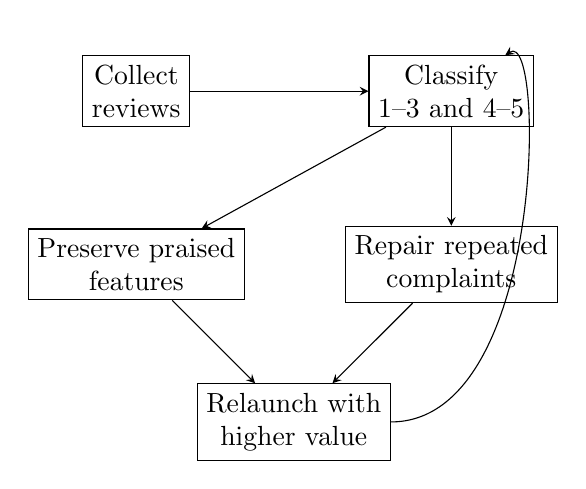
\begin{tikzpicture}[>=stealth]
\node[draw, align=center] (a) at (0,0) {Collect\\reviews};
\node[draw, align=center] (b) at (4,0) {Classify\\$1$--$3$ and $4$--$5$};
\node[draw, align=center] (c) at (4,-2.2) {Repair repeated\\complaints};
\node[draw, align=center] (d) at (0,-2.2) {Preserve praised\\features};
\node[draw, align=center] (e) at (2,-4.2) {Relaunch with\\higher value};
\draw[->] (a) -- (b);
\draw[->] (b) -- (c);
\draw[->] (b) -- (d);
\draw[->] (c) -- (e);
\draw[->] (d) -- (e);
\draw[->] (e) .. controls (5.2,-4.2) and (5.2,0.8) .. (b);
\end{tikzpicture}

A transcript-based reconstruction of Josh's review loop: preserve what customers already praise, repair what they repeatedly dislike, and relaunch the offer at a higher level of value.
\end{figure}

Josh then widens the scale of the same idea. Recalling a line from a billionaire speaker, he says that one need not answer a billion separate questions; one can answer one question that a billion people have. The conceptual move is clean. We pass from isolated transactions to widely shared demand. Scale does not mean doing more of the same thing for no reason; it means attaching the offer to a need that recurs across a large population.

From there the lecture turns once more, now from product design to the use of founder time. Josh says that the move from seven to eight figures came from identifying and delegating MWA tasks---minimum wage activities---and keeping his attention on the few actions that truly moved the business. This is the place where the 80/20 rule enters:
\begin{equation}
Y_{\text{high leverage}} \approx 0.8\,Y_{\text{total}}
\qquad \text{from} \qquad
X_{\text{key}} \approx 0.2\,X_{\text{activities}}.
\end{equation}

Again we should be careful. This is not a theorem about exact proportions. It is a discipline of focus. The lecture's point is that scale comes not merely from effort, but from a sharper distribution of effort.

The host then pauses, praises the value Josh provided, and deliberately resets the scene. That pause matters. It keeps the lecture from becoming an anonymous list of tips. We are meant to feel that one case has yielded its principle, and only then do we go back out into the city.

\section{Bootstrapping, Loss Arithmetic, and Boring Compounding}

The next entrepreneur moves us into residential and commercial solar. The business model is different, but the host keeps the same order of inquiry: industry, scale, method. We hear first that the company operates in fifteen states and then that
\begin{align}
R_{\text{solar,now}} &\approx \$30\,\text{million},\\
R_{\text{solar,target}} &\approx \$100\,\text{million}
\quad \text{within }2\text{ to }3\text{ years.}
\end{align}

The path offered here is bootstrapped rather than venture-backed: flipping sneakers, selling online, learning sales in direct, ordinary environments, and then building a company from scratch. The transcript around the millionaire threshold is slightly garbled, but the substance is clear enough: he attributes his early financial breakthrough to a combination of crypto accumulation, sales success, and entrepreneurship.

What follows is the section's real mathematical center. Asked for the best financial advice he ever received, he gives the old Buffett rule not to lose money and immediately supplies the asymmetry that makes the advice more than a slogan.

\subsection{Question \& Answer}

\paragraph{Question.} Why does boring compounding beat flashy wins?

\paragraph{Answer.} Because large losses damage the compounding process asymmetrically. If wealth falls from \(W_0\) to
\begin{equation}
W_1=(1-L)W_0,
\end{equation}
where \(L\) is the fractional loss, then the gain fraction \(g\) required to recover must satisfy
\begin{equation}
W_1(1+g)=W_0.
\end{equation}
Solving step by step, we find
\begin{align}
g &= \frac{W_0-W_1}{W_1}\\
  &= \frac{L}{1-L}.
\end{align}

The lecture's numerical example is then immediate. For a \(50\%\) drawdown,
\begin{equation}
L=0.5
\qquad \Longrightarrow \qquad
g=\frac{0.5}{0.5}=1=100\%.
\end{equation}

This is the cleanest worked derivation anywhere in the episode. Its meaning is practical rather than decorative: volatility and damage are not symmetric. The deeper the fall, the more violently later growth must work merely to get us back to zero.

The entrepreneur then turns from avoiding loss to accumulating steadily. He cites a rough market-return band
\begin{equation}
r \in [0.08,\,0.10]
\end{equation}
and recommends automation into broad index funds. The standard compounding model is
\begin{equation}
W_n=W_0(1+r)^n,
\end{equation}
and with a fixed recurring contribution \(c\) we obtain
\begin{equation}
W_n=W_0(1+r)^n + c\,\frac{(1+r)^n-1}{r}.
\end{equation}

This reconstruction should be read modestly. The interview itself does not derive the formula. What it does give us is the qualitative picture: steady contributions, long time, and a late steepening of the curve strong enough to change the scale of the outcome.

\begin{figure}[h]
\centering
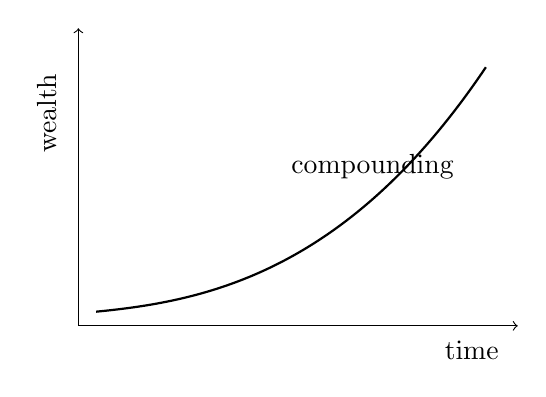
\begin{tikzpicture}[scale=0.9]
\draw[->] (0,0) -- (6.2,0);
\draw[->] (0,0) -- (0,4.2);
\draw[thick] (0.25,0.2) .. controls (1.8,0.35) and (3.8,0.75) .. (5.75,3.65);
\node at (5.55,-0.35) {time};
\node[rotate=90] at (-0.45,3.0) {wealth};
\node at (4.15,2.25) {compounding};
\end{tikzpicture}

A schematic compounding curve of the sort the interview invokes: modest-looking early increments, followed by a visibly steeper late phase once growth itself begins to generate further growth.
\end{figure}

The speaker's practical blueprint is then almost austere. First, make yourself capable of handling money. Second, choose something boring and become excellent at it. Third, scale the craft. Fourth, feed the proceeds into appreciating assets and repeat. The examples of plumbing, roofing, and flooring are used precisely to remove glamour from the story. The lecture wants us to see that durable wealth often emerges from mastery in unromantic domains.

Once again the host pauses, summarizes the value given, and then walks us toward a new kind of scale.

\section{Commercial Real Estate: Scale, Fear, and Incentive Alignment}

Ari's segment raises the absolute scale and changes the sales environment. We are now in commercial real estate, and the speaker is an attorney by training who moved as quickly as he could into the business he expected to be in. The quantitative picture is large, but again it arrives in several non-equivalent units:
\begin{align}
A_{\text{RE}} &= \text{hundreds of millions of dollars},\\
S_{\text{under construction}} &> 10^6\ \text{ft}^2,\\
S_{\text{Tesla-adjacent}} &\approx 600{,}000\ \text{ft}^2,\\
V_{\text{RE,projected}} &\approx \$2.5\,\text{billion}
\quad \text{over the next }4\text{ years.}
\end{align}

What is striking is that, after listing those scales, Ari gives ordinary savers almost the same advice we just heard in the prior segment: index funds, automation, patience, and the long horizon. That echo is part of the lecture's architecture. No matter how glamorous the business gets, the use of surplus capital is described in plain, repetitive terms.

Where Ari differs sharply is in his account of sales. In commercial real estate, he says, clients may speak in the language of return, but beneath that is a fear of losing money or being drawn into a sham. The relevant problem is not merely persuasion. It is fear reduction. Risk controls, real care for the client, visible co-investment, and aligned interests all work on that fear.

The lecture's distinction between fee business and performance business can be stated schematically as
\begin{equation}
\text{manager payoff} \propto \text{performance}
\qquad \text{rather than} \qquad
\text{manager payoff} \propto \text{capital raised}.
\end{equation}

This is a simplified formalization, but it captures the point of the interview. If the manager gets paid for raising money regardless of outcome, mistrust is rational. If the manager gets paid by making money alongside the client, the incentives become legible. Once that alignment is visible, trust stops being a soft moral appeal and becomes part of the business logic.

The host again marks the transition explicitly: Ari has given advice, the experience was worthwhile, and now the lecture will ``keep it rolling.'' That reset carries us away from asset-heavy, trust-heavy real estate and toward the world of venture-backed technology.

\section{Technology Startups, Valuation, and the Team Principle}

Renji's segment begins with surprise and escalation. He is introduced as the founder of one of the largest tech startups in Texas, active in AR, VR, spatial computing, software, and hardware. The metrics fit the venture world:
\begin{align}
C_{\text{raised}} &\approx \$87\,\text{million},\\
V &\approx \$1\,\text{billion}.
\end{align}

A bookkeeping warning is essential here:
\begin{equation}
V \neq R.
\end{equation}
The host asks what the business will generate, but the answer pivots immediately to valuation. This is faithful to startup discourse and potentially confusing unless we keep the categories separate. Renji himself helps by noting that technology companies often trade on higher multiples than ordinary operating businesses.

His more important contribution is the structural one. He says he chose the sector because Meta, Microsoft, Google, and Apple are all pouring enormous capital into it, but he also insists that the goal is not merely to sell to the giants. The aspiration is to build the next one.

\subsection{Question \& Answer}

\paragraph{Question.} What is the blueprint for a startup that survives and scales?

\paragraph{Answer.} Renji's answer comes in a strict order:
\begin{enumerate}
\item Build a product that people actually want.
\item Build the team that can build and improve that product.
\item Find the funding, or the internally generated cash flow, that keeps the team alive long enough to scale.
\end{enumerate}

The order matters. Funding is not first. Fashion is not first. The lecture deliberately opposes the common tendency to jump into whatever looks easy or profitable merely because others are doing it. For Renji, differentiation comes from competence and from the reality of demand. Valuation is then a consequence of structure, not a mystical property bestowed at the beginning.

The host praises the answer and moves on, but the episode is not yet done. The last entrepreneur functions as a final correction to everything we may have been tempted to mythologize.

The final founder tells a story of drifting into high tech almost against his earlier preferences. He disliked computer science, disliked sales, and then found himself at IBM in computer sales. From there came company building in Austin, a first company sold for about \(\$150\) million, then a later company involved in a go-private round of about \(\$7\) billion, and eventually a business with a little over half a billion in revenue and roughly \(2{,}500\) employees:
\begin{align}
X_{\text{first exit}} &\approx \$150\,\text{million},\\
X_{\text{go-private}} &\approx \$7\,\text{billion},\\
R_{\text{later company}} &> \$0.5\,\text{billion}.
\end{align}

But the lecture does not end on those numbers. It ends on a denial: the mythology of the brilliant entrepreneur acting alone is false. The advice is first to know what one is good at, then to surround oneself with people who are strong where one is weak. The scaling secret is not lone genius. It is a durable team with complementary strengths.

That is the right closing gesture. We began with scale as spectacle. We end with scale as organized cooperation.

\section{Summary}

The chapter unfolds as a sequence of numbers translated into mechanisms. The cold open teaches us to distinguish revenue from valuation, earnings from exits, capital raised from assets under management. Josh then gives the first serious operating model: large profits arrive in concentrated windows; premium pricing follows value; value can be built by studying what already works, sorting reviews carefully, and focusing founder time on the few actions that move the business. The solar entrepreneur adds the arithmetic of capital preservation and the steady machinery of compounding. Ari turns scale into a lesson about fear, trust, and incentive alignment. Renji turns it into a lesson about product, team, and funding. The last founder removes the last illusion by insisting that great companies are built by teams, not by legends.

So the lecture's deeper statement is simple. Wealth is not one object, and success is not one trick. We make progress only when we distinguish the scales, identify the mechanism appropriate to each scale, and then follow patiently the chain by which money is earned, protected, compounded, and organized through other people.